
\chapter{序言}
\thispagestyle{empty}

\setlength{\fboxrule}{0pt}\setlength{\fboxsep}{0cm}
\noindent\shadowbox{
\begin{tcolorbox}[arc=0mm,colback=lightblue,colframe=darkblue,title=学习目标与要求]
%kai\textcolor{darkblue}{1.~~对抗学习.} \\ 

\end{tcolorbox}}
\setlength{\fboxrule}{1pt}\setlength{\fboxsep}{4pt}

\section{算法演进之路}

从pc互联网到移动互联网,阿里巴巴电商平台一路高歌猛进,
数据规模,计算能力都发生了天翻地覆的变化;
如图1所示,
\begin{figure}[h]
\centering
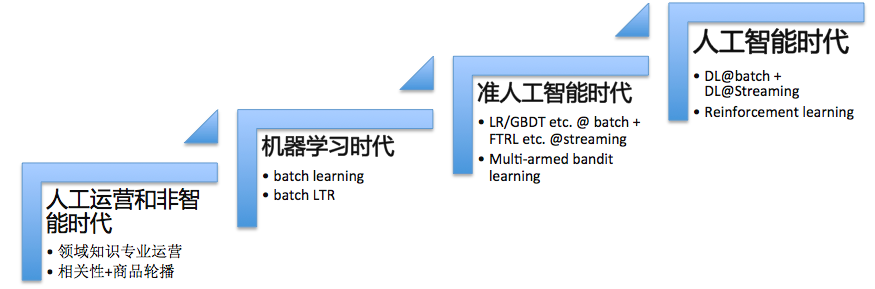
\includegraphics[totalheight=2.0in]{fig/searchAlgoRoadmap.png}
\caption{搜索智能化体系演进图} \label{fig:gansamples}
\end{figure}

\subsection{人工+弱算法时代} 
这个时代的关键词:\textbf{规则 + 轮播}

算法及模型在搜索和推荐系统领域占据统治地位之前,具有领域知识的专业运营和
产品往往充当信息展示规则的制定者,根据主观的判断和对市场的敏锐度来制定
查询词背后的商品展示逻辑。“人工规则”的好处是容易理解和操控,坏处则不言而喻,
随着平台规模的增大,简单规则无法精细的表达人货匹配的效率,并且容易被一些
不良商家利用规则来扰乱市场秩序;实际上,早期的搜索和推荐系统也会运用一些
基本的算法逻辑来保证信息匹配的正确性和人货匹配的公平性,基于传统搜索
引擎技术的相关性模型,保证用户查询词语商品标题的有效匹配;基于商品成交
与否的销售人气指数模型,保证有助于被消费者接受的商品得到更多的展示机会;
另外还有一个就是系统为了保证让更多商家有机会得到展现,设置的按照虚拟下架
周期为参考的轮播因子,即将下架的商品会得到相对较高的展示机会。
$$
	score(item)=1-\frac{ItemOffshelfTime-QueryTime}{secondsOfTwoweek}\times(\frac{docFound}{delta})
$$

这个时代遗留下来几个关键问题需要解决:
\begin{description}
	\item 
\end{description}

\subsection{大规模机器学习时代}
这个时代的关键词:\textbf{big data,offline + shallow model}

随着平台规模的扩大,大规模商家入驻,积极的在平台上打理店铺,发布商品,
相对结构化的商品组织体系,类目结构,属性信息,基于商品为主键的销量的累积,
评论的累积,这些为更好的理解商品积累了重要的原始数据资料;
消费者通过搜索产品的各级页面与平台的互动越来越频繁;
数据的组织形成了以人为主键的结构体系,反馈信号也得以在闭环系统中有效的流转;
所有的这些都为理解用户积累了重要的数据资料。
有效数据的积累为大规模运用机器学习技术解决问题提供了必要的土壤。

这方面各大互联网公司和科研机构,学校公开发表出来的有参考价值的工作有不少,
典型的有价值工作,logistic regression,gbdt; 


\section{业务问题的思考@淘宝搜索} 

\begin{figure}[h]
\centering
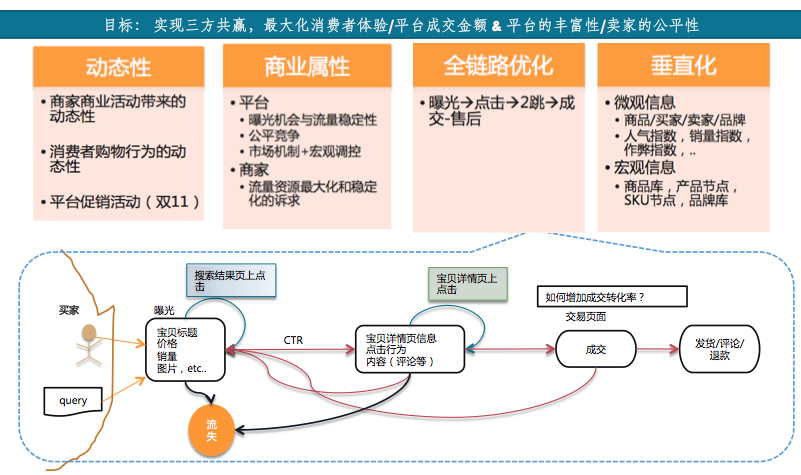
\includegraphics[totalheight=3.0in]{fig/searchProdFea.png}
\caption{电商搜索特性} \label{fig:gansamples}
\end{figure}

淘宝的搜索平台是致力于提供一个一个买家和卖家的公平交易平台;作为一个公平的市场调节员,调整供需平衡,为卖家引导潜在的兴趣用户,以提升其ROI(return on investment),为用户提供满足其需求(user intent)的商品;商业流量下的搜索自然带有其特有的技术特点:

\subsection{动态性}

网页搜索的对象的是分布于各类网站发布的网页,从索引单元上对比,数量上是绝对要远远大于商品搜索的对象集合,如果把每个商品展示页当成是淘宝网站的普通网页的化,表象上讲,商品页面的信息集合应该是网页搜索对象集合的一个子集;网页搜索中的基本对象也存在网页更新,然而淘宝搜索的商品库具有更强的动态性,宝贝的循环搁置,新卖家加入,卖家新商品的推出,价格的调整,标题的更新,旧商品的下架,换季商品的促销,上下架,降价,宝贝图片的更新,销量的变化,卖家等级的提升,商品竞争程度的提升等,都需要淘宝的商品搜索引擎在第一时间捕捉到变化,并及时反映到索引结构中的相应信息单元,而最终的排序环节,这些变化也会动态的融入排序因子,带来排序的动态调整;因此对于商品搜索引擎,要求建立高效的索引更新体系,适应商品类目体系,倒排索引结构,匹配机制的召回逻辑,以及应对商品排序信息及时生效的cache分层机制;

\subsection{全链路优化}

众所周知,相比类似百度这样的网页搜索平台,一个明显的差异是,淘宝搜索平台拥有网购消费者从查询到完成目标商品订单,这样一条完整的行为数据闭合式链路;因此对于用户的一次查询的满意度衡量绝不能止于搜索结果页上看到一个标题相关的商品而发生了点击来判别,post-click之后的商品详情页上的行为,甚至于进入post-pay之后的评论信息都应该成为度量某商品对于某次查询(query)的满意度影响因子;因此,全链路的行为建模会是淘宝搜索体系相比于网页搜索的重要差异之处;既然谈到这点了,再多啰嗦两句,京东也是一家做电子商务的公司,也有着不小的规模,那么如何来看淘宝搜索与京东搜索在全链路优化上的差异呢?从京东模式来看,post-pay环节,由于销售,物流仓储的自营性,可以认为是无差异竞争的;而对于淘宝来说,售后的服务,发货速度,以及纠纷退款等环节是取决于商家与消费者之间的互动来决定的,差异性不言而喻,因此淘宝搜索有必要建立post-pay环节的排序度量因子;

\subsection{商业属性}

电子商务平台的搜索自然具备商业流量的根本属性,商家希望所经营商品通过得到足够的曝光而带来成交;因此,流量资源(曝光)也就成了商家必争之地。搜索排序体系的白盒化和可解释性自然是至关重要。淘宝搜索的ranking,更接近于一个带约束的优化问题,而不是一个简单的排序,优化的目标是最大化平台的成交金额;而约束则是卖家流量分配的诉求;这个环节的涉及到的课题也是电商平台最复杂之处,我会在下面集中阐述下我的一些观点;

\subsection{垂直化}
电子商务搜索属于 vertical search 范畴,相比于网页搜索,对于平台上内容的结构化梳理,以及商业平台上积累的买家,卖家和商品关系数据的挖掘都有更高的要求;因此需要建立 micro analysis 和 macro analysis 双位一体的搜索内容加工体系,宏观分析层面指的是:除了目前已经积累并广泛运用的5级类目之外,完善的商品库建设,spu节点,sku节点,品牌库等,都是必不可少的;微观分析层面则从商品的人气指数,销量指数,作弊指数等角度给出商品自身质量的度量信息;使得搜索结果能够为消费者提供,不仅仅停留在标题相关层面的服务,可以通过合理的宏观分析带来的数据结构化,实现高效的结果查询,通过细致的微观分析,保证优质的商品优先展示给消费者;


\begin{figure}[h]
\centering
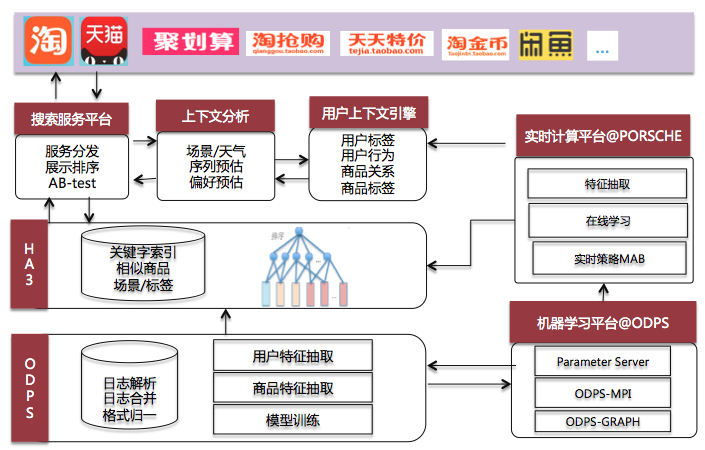
\includegraphics[totalheight=3.0in]{fig/techForBusiness.png}
\caption{智能化助力商业产品} \label{fig:gansamples}
\end{figure}

\section{技术挑战@业务问题} 
\subsection{算法模型} 
像众多互联网企业一样,大数据环境下,基于用户行为建模所面临的技术挑战很多,大家耳熟能详的点列举如下: 
\begin{description}
	\item 投放逻辑带来的数据bias对行为建模的影响
	\item 用户行为数据的稀疏性
	\item 因果关系的模糊性
	\item 用户行为的时效
	\item 行为个性化和非个性化 unified ranking
	\item Cold start modeling
	\item 多样性与精确性的tradeoff (过度个性化)
	\item 长短期个性化融合
\end{description}

\subsection{工程技术} 
随着数据规模的指数级增长,完成复杂数据建模对于工程技术体系的挑战也是不言而喻: 
\begin{description}
	\item 千亿行为和关系数据存储、实时更新和查询
	\item 翻页陷阱
	\item Cache机制
	\item 分级实时体系(数天/小时/秒/ms)
\end{description}

\subsection{效果评估}
效果评估是保证体系迭代朝正向发展的关键保障。
\begin{description}
	\item 模型正确性评估
	\item AB体系下分群评估
	\item 社会化评测
\end{description} 



\begin{thebibliography}{99}
\addcontentsline{toc}{chapter}{\protect\numberline{}{\hspace{-1.5em}参考文献}}
\markboth{参考文献}{参考文献}
\bibitem{1} Bilinear+LinUcb的个性化主题推荐, http://www.atatech.org/articles/67847
\bibitem{2} 依托搜索技术的个性化平台之路, http://www.atatech.org/articles/13748
\bibitem{3} 用户意图预估之实时意图篇, http://www.atatech.org/article/detail/12636/152
\bibitem{4} 知人知面需知心——论人工智能技术在推荐系统中的应用,http://geek.csdn.net/news/detail/112318
\bibitem{5} Google, Ad Click PredictionL a View from the trenches. pCTR使用LR,通过
FTRL Proximal 算法实现在线模型更新,频率学派,写的很细致,也有工程细节
\bibitem{6} Bing, Web-Scale Bayesian Click-through Rate Prediction for sponsored 
Search Advertising in Microsoft‘s Bing Search Engine。 Online Bayesian Probit Regression,贝叶斯学派,涉及采样算法的模型
\bibitem{7} Facebook, Practical Lessones from Predicting Clicks on Ads Clicks 
on Ads at facebook。 DT+LR。 和GBDT非常类似,不同之处在于用LR重新训练了每棵树投票的权重,
人气很旺的xgboost,在这一块也是做了优化,利用二阶导数信息得到更快收敛的步长。 缺点是
处理不了高纬度特征,处理连续值特征有优势。
\bibitem{8} 我所经历的大数据平台发展史(三):互联网时代 • 上篇, http://www.infoq.com/cn/articles/the-development-history-of-big-data-platform-paet02, 
\bibitem{9} Fast and Reliable Online Learning to Rank
for Information Retrieval, https://khofm.files.wordpress.com/2013/04/thesis-katja-hofmann-online-learning.pdf
\bibitem{10} Dawei Yin, etc.., Ranking Relevance in Yahoo Search, KDD'16 
\bibitem{11} C.J.C. Burges, FromRankNettoLambdaRanktoLambdaMART: An overview, Technical 
report, Microsoft Research 2010
\bibitem{12} Z. Cao, T. Qin, etc.., Learningtorank: from pairwise approach to listwise approach, ICML'07 
\bibitem{13} A. Dong, Y. Chang, etc.., Towards recency ranking in web search. In WSDM'10. 
\bibitem{14} AI在双11中的个性化搜索和决策实践
\bibitem{15} 电子交易欺诈层出不穷,如何用深度学习系统步下天罗地网
\bibitem{16} 场景驱动结合软硬创新
\bibitem{17} 一文综述所有用于推荐系统的深度学习方法
\bibitem{18} 卷积网络视角下的大信息过滤理论
\bibitem{19} A/B测试那些事 
\bibitem{20} 文本分类的选择:词袋模型 vs. 深度序列模型
\bibitem{21} 深度报告: “数据革命” 终极方向是人工,金融/汽车最快落地
\bibitem{22} 当机器学习遇上复杂网络
\bibitem{23} 机器学习在工业应用中的新思考
\bibitem{24} 深度学习在搜索和推荐领域的应用
\bibitem{25} 知人知面需知心--人工智能技术在推荐系统中的应用




\end{thebibliography}

 
